\documentclass[10pt,a4paper]{article}
\usepackage[utf8]{inputenc}
\usepackage[german]{babel}
\usepackage[T1]{fontenc}
\usepackage{amsmath}
\usepackage{amsfonts}
\usepackage{amssymb}
\usepackage{graphicx}
\usepackage{float}
\usepackage{hyperref}
\usepackage{longtable}

\title{\textbf{Sister Shift} \\ Konzept \\ erstellt von}

\author{David Jovanoski & Marco Schröder}
\begin{document}
\begin{figure}

\includegraphics[scale=1]{Bilder/Logo_TH-Koeln_RGB_17pt.jpg}
\end{figure}
\maketitle
\tableofcontents
\listoffigures
\section{Exposé}
\subsection{Nutzungsproblem}
Eine Stationsleitung in einem Krankenhaus stellt sich regelmäßig dem Problem, einen möglichst ausgeglichenen und fairen Dienstplan für Krankenpfleger zu erstellen. Dabei müssen gesetzliche aber auch Krankenhaus spezifische Richtlinien eingehalten werden. Außerdem ist es aus Gründen der Moral von den Arbeitnehmern sehr wichtig, die Wünsche der Mitarbeiter zu berücksichtigen. Diese beinhalten Urlaubs aber auch Dienstwünsche. Abwesenheit ist im Gesundheitswesen immer eine kritische Angelegenheit. Es kann durch plötzliche Krankheitsfälle oder sonstigen Ereignissen im Privatleben eines Arbeitnehmers zu Dienstausfällen kommen. Auf diese passend und schnell zu reagieren ist sehr schwer und umständlich. Außerdem ist ein Dienstplan nur sehr umständlich vom Arbeitnehmer zu individualisieren.
\subsection{Zielsetzung}
Das Projekt soll die im Nutzungsproblem dargestellte Aufgabe der Stationsleitung weitestgehend automatisieren. Es soll richtlinienkonform ein Dienstplan erstellt werden. Bei diesem Dienstplan soll auf Basis der Wünsche, ein möglichst Fairer Plan erstellt werden. Falls eine Person plötzlich ausfällt, soll automatisch ein Ersatz gefunden werden. Dabei wird wieder auf Richtlinien und Wünsche geachtet. Zusätzlich soll der Arbeitnehmer die Möglichkeit der Individualisierung seines Dienstplanes haben.
\subsection{Verteilung der Anwendungslogik}
Für die Berechnung des Dienstplans, sind zunächst die Richtlinien des zuständigen Krankenhauses, einzupflegen. Die Mitarbeiter müssen in einem gewissen Zeitintervall ihre Wünsche äußern. Falls es zu Konflikten im Dienstplan kommt, soll es in Abhängigkeit von Eigenschaften der Personen oder Vorhergegangenen Dienstplänen zu einer Entscheidung kommen. Bei Personenausfällen sollen freie Mitarbeiter prioritätsbezogen benachrichtigt werden und je nach Antwort, der Dienstplan der betroffenen Personen angepasst werden. Eine Möglichkeit zum Einsehen und Tauschen von Diensten muss gegeben sein.
\subsection{Gesellschaftlicher Aspekt}
Den Krankenschwestern eines Krankenhauses wird aufgrund der besonderen Fairness, der vereinfachten Planung und Individualisierbarkeit geholfen eine hohe Arbeitsmoral beizubehalten. Die Zu-friedenheit der Mitarbeiter ist eines der wichtigsten Ziele in einer Organisation. Da das Planen und umstrukturieren weitestgehend als Aufgabe der Stationsleitung entfällt, hat diese nun mehr Zeit sich mit anderen Problemen der Mitarbeiter zu befassen und sich mehr den Patienten und deren Bedürfnissen zuzuwenden.
\section{Domänenrecherche}
\begin{figure}[H]
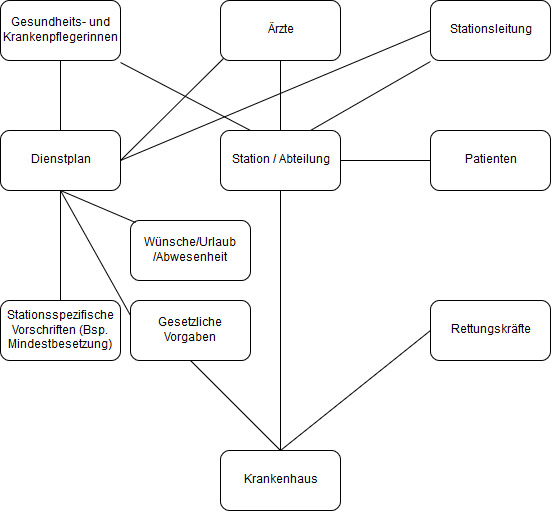
\includegraphics[scale=0.6]{Bilder/Domaenenmodell.jpg}{\centering}
\caption{Domänenmodell}
\end{figure}
\subsection{Krankenhaus}
Ein Krankenhaus zählt zu den komplexesten Organisationen der modernen Zeit. In diesem müssen täglich große Organisationsleistungen vollbracht werden, um den täglichen Routinebetrieb zu bewältigen und die Funktionsfähigkeit des Krankenhauses aufrecht zu erhalten. Eine funktionierende Organisation ist im Gesundheitswesen sehr wichtig. Das Krankenhaus ist daher eine sehr komplexe Organisation, da es mehrere Funktionen gleichzeitig zu bedienen hat, welche sich gegenseitig ergänzen und nicht behindern dürfen. Es ist das Zentrum der Gesundheitsversorgung, Aufenthaltsort für Patienten, Arbeitgeber für sehr viele Beschäftigte, Einrichtung der Aus- und Weiterbildung,  eine Institution in der öffentliche und private Forschung betrieben wird, und es muss in seiner Leistungserbringung die Interessen sehr unterschiedlicher Stakeholder-Gruppen berücksichtigen wie Patienten, Politik, Verwaltung, andere Institutionen der Gesundheitsversorgung, Gesetzeslagen, Wissenschaftliche Communities, und Fachgesellschaften. (vgl. Ralph Grossmann und Hubert Lobnig: Organisationsentwicklung im Krankenhaus – Grundlagen und Interventionskonzepte) 
Die optimale Planung von Einsatzzeiten der verschiedensten Mitarbeiter ist eine der wichtigsten Kernaufgaben in der Organisation. In diesem Bereich sind zum einen gesetzliche, aber auch aus dem Gesundheitswesen spezifische Gesetze und Vorgaben einzuhalten. Die detaillierte Planung der Besetzung einer Station übernimmt im Regelfall die Stationsleitung. Auf verschiedenen Stationen gibt es Individuelle Unterscheidungen, was die Dienstzeit und die Besetzung angehen. Auf der Station der Notaufnahme zum Beispiel gibt es vier Arten von Diensten. Das sind die Frühdienste, Spätdienste, Nachtdienste und Zwischendienste. Die Besetzung unterscheidet sich von Schicht zu Schicht. Im Früh- und Spätdienst müssen mindestens fünf Krankenpfleger gleichzeitig Dienst haben. Im Nachtdienst reichen drei. In diesem Bereich gibt es allerdings die Ausnahme, dass ein Pfleger einen Dienstwechsel in der laufenden Arbeitswoche hat. Ist dies der Fall, muss der Pfleger als Übergang einen Zwischendienst absolvieren, und im Frühdienst reicht eine Besetzung von vier Krankenpflegern aus. Da nach der Beendigung eine Ruhezeit von mindestens 11 Stunden eingehalten werden muss, ist ein Wechsel von Spätdienst auf einen Frühdienst nicht möglich.
Es existiert eine Aufgabenteilung zwischen den Krankenpflegern. Ein Krankenpfleger arbeitet entweder internistisch oder in der Chirurgie. Während der Erledigung des Routinebetriebs übernimmt ein Krankenpfleger des aktiven Dienstes die Funktion des sogenannten “Springers”. Dies bedeutet, dass dieser Mitarbeiter bei Bedarf in dem jeweiligen Bereich aushelfen kann. 
In einem Krankenhaus gibt es eine Vielzahl von unterschiedlichen Personalkräften. Es gibt Vollzeit-, Teilzeitkräfte, Minijobber und Werksstudenten. Jede Art dieser Personalkräfte hat eigene Vorgaben zu Einsatzzeiten und Vergütung. Dies muss bei der Personalplanung von der Stationsleitung stets beachtet werden. 
Tritt nun der Fall eines spontanen Personalausfalls ein, so müssen sich die eingeteilten Mitarbeiter selbstständig untereinander absprechen und in Zusammenarbeit mit der Stationsleitung einen Ersatz für den entfallenden Mitarbeiter finden.
Sonstige Besonderheiten zur Personalplanung existieren ebenfalls bei der Dienstplanung an Feiertagen. Die Stationsleitung hat die Aufgabe die Dienste an Feiertagen fair unter allen verfügbaren Mitarbeitern aufzuteilen. Die Krankenpfleger haben allerdings auch die Möglichkeit Wünsche zu äußern, an welchen Feiertagen ein Dienst besser passen würde und an welchen nicht. 
\subsection{gesetzliche Rahmenbedingungen}
Gesetzliche Bestimmungen zum Schutz der Arbeitnehmer müssen natürlich auch im Gesundheitswesen eingehalten werden. Laut dem Arbeitszeitgesetz (ArbZG) muss die Mindestruhezeit für einen Arbeitnehmer nach der täglichen Arbeitszeit 11 Stunden betragen. Die Dauer der Ruhezeit darf in Krankenhäusern auf 10 Stunden verkürzt werden. Dies darf aber nur unter der Bedingung geschehen, dass jede Verkürzung der Ruhezeit durch eine Mindestruhezeit von 12 Stunden ausgeglichen wird. Es ist zu beachten, dass jeder Arbeitnehmer mindestens 15 freie Sonntage im Jahr hat. 
Der Arbeitgeber ist verpflichtet jeder Kraft nach Einsatz an einem Sonntag oder Feiertag einen Ersatzruhetag in den folgenden zwei Wochen zu gewähren. Jeder Arbeitnehmer hat das Recht auf 24 Urlaubstage in einem Kalenderjahr. (vgl. Arbeitszeitgesetz § 5 Ruhezeit, § 11 Ausgleich für Sonn- und Feiertagsbeschäftigung, Bundesurlaubsgesetz § 3 Dauer des Urlaubs)
Bei Jugendlichen und Auszubildenden unter 18 Jahren, muss die Ruhezeit laut Jugendarbeitsschutzgesetz mindestens 14 Stunden betragen. (vgl. Jugendarbeitsschutzgesetz §14 Nachtruhe). Jugendliche dürfen maximal zwei Samstage und zwei Sonntage im Monat Arbeiten. Zusätzlich ist vorgeschrieben, dass sie nicht am 24 und 31 Dezember arbeiten dürfen. Die Beendigung des Arbeitstages muss vor einem Berufsschultag um spätestens 20 Uhr erfolgen. Jeder angestellte Jugendliche hat das Recht auf 25 Urlaubstage in einem Kalenderjahr (vgl. Jugendarbeitsschutzgesetz §17 Sonntagsruhe, §16 Samstagruhe, §18 Feiertagsruhe, §19 Urlaub, §14 Nachtruhe).
\section{Stakeholderanalyse}
\begin{longtable}{ |  p{3cm} |  p{3cm} | p{3cm} | p{3cm} |}
    \hline
    Bezeichnung & Bezug zum System & Objektbereich & Erfordernis/Erwartung \\ \hline
    Gesundheits-und Krankenpfleger & Interesse & Erstellung fairer Dienstpläne | Wunschäußerung | Automatisierte Ersatzfindung bei Personalausfall | Individualisierbarkeit des Dienstplans & Dienstpläne sind Fair gestaltet und Wünsche werden so gut wie möglich miteingebunden | Das System automatisiert das finden von Ersatzpersonal im Falle eines Personalausfalls | Individualisierbarkeit des Dienstplans ist nach der Erstellung dieses mit gewissen Einschränkungen möglich | Das System ist einfach zu verstehen und zu bedienen \\ \hline
    Stationsleitung & Interesse & Automatisierte Diensplanerstellung | Ersatzfindung bei Personalausfall | Individualisierbarkeit des Dienstplans & Faire Dienstpläne werden automatisch, ohne viel Zutun von Mensch gesteuertem Input generiert | Mitarbeiter können Ihren Dienstplan selbstständig Individualisieren | Das System automatisiert das finden von Ersatzpersonal im Falle eines Personalausfalls | Unterstützung beim Personalmanagement + Zeitgewinnung für andere Aufgaben | Das System ist einfach zu verstehen und zu bedienen | Benachrichtigung bei etwaigen Personalausfällen \\ \hline
    Patient & Interesse & Druchgängige Zuteilung einer Pflegekraft auf die entsprechende Station  & Es ist permanent die richtige Besetzung an Pflegekräften eingeteilt um bei etwaigen Bedürfnissen der Patienten helfen zu können \\
    \hline
    Krankenhaus & Anspruch & Umfassende Unterstützung der Dienstplanerstellung  & Dienstpläne sind zuverlässig und mit den Bedingungen in einem Krankenhaus vereinbar \\
    \hline
    Politik & Anrecht & Einhaltung gesetzlicher Vorschriften | Faire Behandlung der Arbeitnehmer in Bezug auf Einsatzplanung  & Die Dienstpläne müssen nachweisbar die Gesetzesvorlagen einhalten \\
    \hline
    Fachgesellschaft & Anteil & Automatisierte Dienstplanerstellung und Reaktion auf Abwesenheitsmeldung | Individualisierbarkeit  & Das System muss auch in extrem Situationen (Viele Abwesenheitsvorfälle o.ä.) einen vernüftigen und fairen Dienstplan generieren | Individualisierbarkeit muss mit Bedingungen konform sein | Ersatzfindung im Falle von Personalausfall muss problemlos funktionieren \\
    \hline
    Dienstleistungs- gesellschaft (Zeitarbeitsfirmen) & Interesse & Heranziehen von externem Personal bei Personalmangel  & Rechtzeitiges Einplanen der externen Personalkräfte, um ordnungsgemäße Zeitarbeitsverträge abschliessen zu können \\
    \hline
\end{longtable}
\section{Anforderungen und Erfordernisse}
\subsection{Erfordernisse}
[E01] Als Gesundheits- und Krankenpfleger in einem Krankenhaus muss man persönlichen Zugriff auf die aktuellen Dienstpläne haben, um die jeweiligen Arbeitszeiten in Erfahrung zu bringen
[E02] Die Stationsleitung muss die gesetzlichen und Krankenhaus spezifischen Vorgaben zu Dienstplänen von Gesundheits- und Krankenpflegern wissen, um korrekte Dienstpläne erstellen zu können
[E03] Als Gesundheits- und Krankenpfleger muss man eine E-Mail-Adresse oder Telefonnummer besitzen, um über Änderungen am Dienstplan informiert zu werden, und um im Falle eines Personalausfalls einen Ersatz zu organisieren
[E04] Die Gesundheits- und Krankenpfleger müssen eine Möglichkeit der Kommunikation mit dem Verantwortlichen der Dienstplanerstellung haben, um persönlich Wünsche zur Einsatzzeit oder Urlaub mitzuteilen
[E05] Es müssen in jeder Schicht, zu jedem Tag ausreichend Gesundheits- und Krankenpfleger eingeteilt sein, um eine gute Versorgung der Patienten zu gewährleisten
\subsection{Anforderungen}
[A01] Das System muss Gesundheits- und Krankenpflegern die Möglichkeit bieten Ihren aktuellen Dienstplan einzusehen
[A02] Das System muss bei der automatischen Erstellung der Dienstpläne alle gesetzlichen und Krankenhaus spezifischen Gesetze und Regelungen beachten und einhalten
[A03] Das System muss jeden Mitarbeiter auffordern eine valide Kontaktmöglichkeit zu hinterlegen
[A04] Das System sollte den Gesundheits- und Krankenpflegern die Möglichkeit bieten persönliche Wünsche zur Einsatzplanung vor der Dienstplanerstellung an dieses mitzuteilen
[A05] Das System muss fähig sein, einen umfassenden Dienstplan für jeden Tag und mit Berücksichtigung jeglicher Schicht, und (soweit wie möglich) der individuellen Wünsche der Mitarbeiter automatisch zu generieren
[A06] Das System muss leicht verständlich und gut bedienbar sein, damit auch ältere Gesundheits- und Krankenpfleger schnell den Gebrauch dieses lernen
[A07] Das System muss den Mitarbeitern die Möglichkeit bieten, eine Abwesenheit zu hinterlegen
[A08] Sobald eine Abwesenheitsmeldung vorliegt, muss das System fähig sein, automatisch einen Ersatz zu organisieren und einzuteilen
[A09] Ist ein Ersatz für einen Personalausfall gefunden und eingeteilt, so muss das System die Dienstpläne der betroffenen Mitarbeiter automatisch anpassen, und die betreffenden Personen + die Stationsleitung über die Änderungen benachrichtigen
[A10] Falls kein Mitarbeiter aus dem eigenen Krankenhaus als Ersatz bei Personalausfall einspringen kann, soll das System bei externen Firmen Personal für den betroffenen Zeitraum anfragen
[A11] Das System muss den Gesundheits- und Krankenpflegern nachdem ein Dienstplan generiert wurde die Möglichkeit bieten, untereinander mit Hilfe des Systems Schichten zu tauschen
[A12] Falls ein Schichten-Tausch angestrebt wird, darf das System nur Tausche zulassen, welche die gesetzlichen und Krankenhaus spezifischen Gesetze und Vorgaben nach dem Vollziehen dieser, immer noch erfüllen
[A13] Das System muss der Stationsleitung die Möglichkeit bieten, Aspekte und Kenngrößen zu dem zu erstellenden Dienstplan festzulegen 
\section{Zielhierarchie}
\subsection{Strategische Ziele}
Das System soll die Stationsleitung in einem Krankenhaus entlasten. Es soll die Aufgabe übernehmen faire Dienstpläne für jeden Mitarbeiter zu erstellen. Es muss alle gesetzlichen und domänenspezifische Vorschriften bei der automatisierten Erstellung dieser einhalten. Das System kann Wünsche bezüglich Einsatzzeiten der Arbeitnehmer mit in die Planung der Dienstpläne einfließen lassen. Die “faire” Einteilung der Gesundheits- und Krankenpfleger muss auf vorausgegangen Schichten, Anzahl von Einsätzen an einem Wochenende, spezifischen Wünschen und einer ausgewogenen Balance aus Früh-, Spät-, Zwischen-, und Nachtschichten basieren. Die Stationsleitung soll vor der automatisierten Erstellung Rahmenbedingungen (Anzahl Personal, Schichtdauer, Personalspezifizierungen) für den zu erstellenden Dienstplan festlegen. Das Tauschen von Schichten untereinander soll von den Gesundheits- und Krankenpflegern eigenständig durchführbar sein. Das System darf nur Schichten zum Tausch zulassen, bei denen ein Tausch nicht zur Verletzung einer domänenspezifischen oder gesetzlichen Vorgabe führt. Zusätzlich soll das System das Organisieren von Ersatzpersonal bei Personalausfall automatisieren. Kommt es zu einem Personalausfall sollen die Arbeitnehmer die Möglichkeit haben, die Abwesenheit selbstständig dem System mitzuteilen. Liegt eine Abwesenheitsmeldung vor, sollen alle verfügbaren Mitarbeiter, welche an der betroffenen Schicht selbst nicht eingeteilt sind, benachrichtigt werden, dass ein Personalausfall zu einer bestimmten Schicht vorliegt. Die Gesundheits- und Krankenpfleger sollen dann die Möglichkeit besitzen, die betreffende Schicht zu übernehmen. Falls dieser Fall eintritt, soll das System automatisch den Dienstplan des betreffenden Mitarbeiters anpassen. Die genannten Ziele sind bis zum 20.01.2019 umzusetzen. 
\subsection{Taktische Ziele}
Das System soll entlang des menschzentrierten Entwicklungsprozesses entwickelt werden und muss auf den sieben Grundsätzen der Dialoggestaltung aufbauen. Eine gute Benutzbarkeit des Systems muss gegeben sein. 
\subsection{Operative Ziele}
Die Umsetzung der automatisierten Dienstplanerstellung muss mit Hilfe einer geeigneten verteilten Anwendungslogik und passenden Algorithmen realisiert werden. Der Austausch von Schichten ist durch Benutzerkontoinformationen und Überprüfung der Vorgaben aus der Dienstplanerstellung zu realisieren.  Die automatisierte Ersatzpersonalplanung muss ebenfalls alle Vorgaben aus der Dienstplanerstellung beachten und ist durch ein Benachrichtigungsverfahren zu realisieren. Die Verantwortliche Person der Personalplanung soll nach Ersatzfindung ebenfalls eine Benachrichtigung erhalten.
\section{Marktrecherche}
\subsection{Allgemein}
Ein Dienstplan bildet die Grundlage der Personaleinsatzplanung. Dienstpläne werden in privaten Unternehmen, Einrichtungen und Institutionen des öffentlichen Sektors, Sicherheitsbehörden oder auch in sozialen Bereichen wie der Pflege verwendet. Ziel ist die optimale und effektivste Verwendung des Personals, um die jeweilig aufkommenden Aufgaben zu bestmöglich zu erfüllen. Dabei müssen rechtliche Grundlagen und Bestimmungen stehts bewahrt werden. 
Viele Unternehmen und Behörden fangen an von der klassischen Weise mittels Vordruckes, auf moderne Software zu Erstellung von Dienstplänen zu setzen. Durch Verwendung von Software können Planungsfehler und Fehlkalkulationen vermindert werden. Diese Tatsache ist besonders in Berufsfeldern wie der Pflege wichtig. Software für die Erstellung von Dienstplänen reicht von open-source bis hin zu monatlich zu bezahlenden Produkten. In vielen Unternehmen wird allerdings auch nur Microsofts Excel zu Erstellung der Dienstpläne verwendet. (vgl. Papershift GmbH: Dienstplan (HR-Lexikon))
Beim Erstellen eines Dienstplans übt ein Arbeitgeber das ihm zustehende Weisungsrecht gegenüber dem jeweiligen Arbeitnehmer aus. Es gibt keine Regelungen bezüglich eines Dienstplans, aber dennoch muss vor allem das Arbeitsgesetz vom Arbeitgeber beachtet werden. Dies gilt zum Beispiel für die zulässige Arbeitszeit pro Tag, die einzuhaltenden Pausen und vieles mehr. Zusätzlich sind Branchenspezifische Vorschriften zu beachten. (vgl. JuraForum.de-Redaktion: Dienstplan erstellen: Gesetzliche Regelung & Rechte des Arbeitnehmers)
Durch Verminderung von Fehlern und Einhaltung gesetzlicher Rahmenbedingungen bietet sich für Software, welche die Erstellung und Planung von Dienstplänen unterstützt große Chancen aktiv am Markt teilzunehmen. Viele open-source Softwareprodukte stoßen schnell an Ihre Grenzen und erfordern andernfalls ein fortgeschrittenes Verständnis dieser Software. (vgl. Papershift GmbH: Dienstplan (HR-Lexikon))
Durch die genannten Faktoren ist ersichtlich, dass Software, welche einen User effizient und einfach unterstützt einen Dienstplan zu organisieren/zu erstellen großes Potential hat. 
Da es am Markt bereits viele open-source und einige Kostenpflichtige Softwareprogramme für diesen Zweck gibt, ergibt sich das Risiko, nicht aus der Masse hervorzustechen. Ein Alleinstellungsmerkmal im Vergleich zur Konkurrenz ist in diesem Fall sehr wichtig. Die Entwicklung in diesem Markt ist sehr stabil, da immer mehr Unternehmen und Behörden Software zu Erstellung/Planung von Dienstplänen benutzen.
\subsection{Wettbewerb}
Der größte Wettbewerber in diesem Markt ist die Papershift GmbH. Diese bietet verschiedenste Dienstleistungen an. Diese umfassen das Erstellen (auch automatisiert) und Bearbeiten von Dienstplänen, das Verwalten von Abwesenheit, Zeiterfassung, und den Zugriff von jedem Gerät. Zusätzlich werden ein einfaches Userinterface und eine starke Einbindung der Mitarbeiter in die Planung angeboten. Diese umfassenden Dienstleistungen stellt die Papershift GmbH mit monatlichen Kosten pro Mitarbeiter in Rechnung.
Ein weiterer Wettbewerber ist die VEGA Software GmbH Softwarelösungen für soziale Einrichtungen. Dieser bietet ebenfalls eine Dienstplan- und Personalmanagement-Software an, welche allerdings mehr auf soziale Einrichtungen, wie Pflegeheime, Hochschulen oder auch Kliniken zugeschnitten ist. Das Angebot umfasst das manuelle Erstellen von Dienstplänen und eine hohe Benutzerfreundlichkeit. Es können verschiedenste Informationen, wie Name, Vorname, Qualifikation jedes Mitarbeiters, Ein- und Ausgangssaldo jedes Mitarbeiters, Soll- und Ist-Arbeitszeit jedes Mitarbeiters, Abrechnungsstatus jedes Mitarbeiters, Alle Dienste und Ausfälle, Vor- und Folgezeitraum des Dienstplans, Wochensummen und/oder Wochensalden, Prüfung der Arbeitszeitgesetze, Prüfung der freien Tage, Prüfung freies Wochenende, Besetzungsanalyse nach Diensten oder Eigendefinition, und Besetzungsanalyse nach Leistungsaufkommen abgerufen werden. Die Bezahlung erfolgt auch bei diesem Softwareangebot gestaffelt nach jedem Mitarbeiter. (vgl. Softguide der Softwareführer: NEXUS/ Dienstplan & NEXUS/ PERSONALMANAGEMENT)
\subsection{Potential für neue Software}
Papershift bietet eine Menge an Komfort und Unterstützung für die Personalplanung an. Allerdings gibt es in manchen Branchen spezielle Problemstellungen, welche von Papershift nicht abgedeckt werden, da die Gesellschaft mit Ihrem Produkt eine breite Masse an verschiedensten Unternehmen ansprechen möchte. Branchenspezifische Probleme können durch besser zugeschnittene Software abgedeckt werden. Ein Aspekt dafür wäre das Finden von Ersatz bei spontanem Personalausfall im Gesundheitswesen. Die Ersatzfindung muss möglichst schnell erfolgen und es gelten besondere Regelungen.
Die Softwarelösung der VEGA GmbH ist mehr auf die Branche der sozialen Einrichtungen zugeschnitten, und bietet daher auch viel mehr spezifische Informationen zu den jeweiligen Dienstplänen. Allerdings müssen die Dienstpläne alle manuell angelegt und verwaltet werden. Eine automatisierte Erstellung der Dienstpläne würde die entsprechenden Mitarbeiter in den jeweiligen Branchen sehr entlasten.
Bei beiden Softwareanwendungen kann zwar die Abwesenheit eines Mitarbeiters vermerkt und eingesehen werden, aber es wird nicht aktiv beim Organisieren eines Ersatzes geholfen. Zusätzlich bietet keine der beiden Anwendungen dem Arbeitnehmer selbst die Möglichkeit auf Individualisierung des Dienstplanes nach dem Erstellen dieses. 
\subsection{Fazit}
Durch die Spezialisierung auf die Branche Krankenhaus gelten für die Dienstpläne, welche durch die geplante Software automatisiert erstellt werden sollen, bestimmte Anforderungen. Diese sind sowohl durch die Krankenhäuser selbst, als wie auch durch den Gesetzgeben definiert. Zusätzlich treten bei der Planung der Gesundheits- und Krankenpflegerinnen in Krankenhäusern spezielle Probleme auf, wenn spontane Personalausfälle auftreten. Dieses Alltagsproblem muss durch die geplante Software ebenfalls behandelt werden (Unterstützung der Ersatzfindung). Da im Leben selten etwas im Voraus planbar ist, und Gesundheits- und Krankenpflegerinnen auch meist an Wochenenden arbeiten, ist es wichtig einen Dienstplan im Nachhinein noch zu individualisieren, um auf sonstige Ereignisse im Privatleben reagieren zu können. Am besten passiert dies unter den Mitarbeitern selbst, damit die Stationsleitung sich wichtigeren Aufgaben widmen kann. Da es selbst in der Branche „Krankenhaus“ noch viele Spezialisierungen gibt, ist es wichtig Einstellungen (Schichtdauer, Besetzung) vor dem automatisierten Erstellen eines Dienstplanes festzulegen. Schichtpläne sollten also Abteilungsabhängig erstellbar sein
\section{Alleinstellungsmerkmale}
\subsection{Automatisierte Dienstplanerstellung mit Spezialisierung auf die Branche Gesundheitswesen (im Detail Krankenhäuser) }
Der größte Wettbewerber am Markt, möchte eine breites Spektrum an Kunden für sein Produkt gewinnen. Zwar gibt es Unterteilungen in Branchen, dennoch fällt die Spezialisierung sehr grob aus. Im Bereich Gesundheitswesen bietet der größte Konkurrent, nur das zusätzliche Feature an, den Mitarbeiten im Dienstplan eine Tätigkeit zuzuweisen. Bei der Anwendung Sister-Shift ist die Spezialisierung im Detail auf die Organisation in einem Krankenhaus zugeschnitten. Verschiedenste gesetzliche aber auch aus dem Gesundheitswesen wichtigen Vorschriften, werden bei der Erstellung der Dienstpläne berücksichtigt. Zusätzlich unterscheiden sich die Bedingungen und Schichten in den verschiedenen Abteilungen eines Krankenhauses zum Teil sehr stark. Aus dem Grund ermöglicht die Anwendung, das Erstellen von abteilungsspezifischen Dienstplänen. Es gibt zwar Branchenspezifische Dienstplanungssoftware, bei diesen ist die Erstellung der Dienstpläne allerdings nicht automatisiert.
\subsection{Handling von unerwarteten Mitarbeiterausfällen}
Ist ein Dienstplan einmal festgelegt, so basiert dieser auf der Einteilung aller verfügbaren Mitarbeiter. Wenn nun ein Mitarbeiter aus den verschiedensten Gründen nicht zu seiner Schicht erscheinen kann, so muss ein Ersatz gefunden werden. Dies ist vor allem im Gesundheitswesen unerlässlich. Die Wettbewerber am Markt, bieten zwar die Möglichkeit Abwesenheit zu notieren, aber unterstützen die Ersatzfindung nicht weiter. Hier kommt das Alleinstellungsmerkmal von Sister-Shift zum Tragen. Die Anwendung ermöglicht es Gesundheits- und Krankenpflegerinnen Ihre Abwesenheit selbstständig dem System mitzuteilen. Das System organisiert daraufhin automatisiert einen Ersatz und passt die Dienstpläne der betroffenen Gesundheits- und Krankenpflegerinnen an.
\subsection{Individualisierbarkeit ausgehend vom Arbeitnehmer}
Begründung: Die Moral und gute Arbeitsstimmung der Mitarbeiter sind das wichtigste Gut in einer Organisation. Aus diesem Grund legt Sister-Shift großen Wert darauf, die Dienstpläne so fair wie möglich zu gestalten. Da manche Ereignisse aus dem Privatleben aber nur schwer planbar sind, bietet die Anwendung den Gesundheits- und Krankenpflegerinnen die Möglichkeit, auch nach dem Erstellen des Dienstplans, diesen weiter zu individualisieren und anzupassen. Sister-Shift bietet den Mitarbeitern die Möglichkeit untereinander, selbstständig Schichten zu tauschen, sofern alle gesetzlichen und internen Vorgaben nach dem Wechsel erfüllt bleiben. Der jeweilige Abteilungsleiter wird nach erfolgreichen Tauschen nur über die geänderte Personalbesetzung informiert und muss keine weitere Arbeit in die Personalplanung investieren.
\begin{figure}
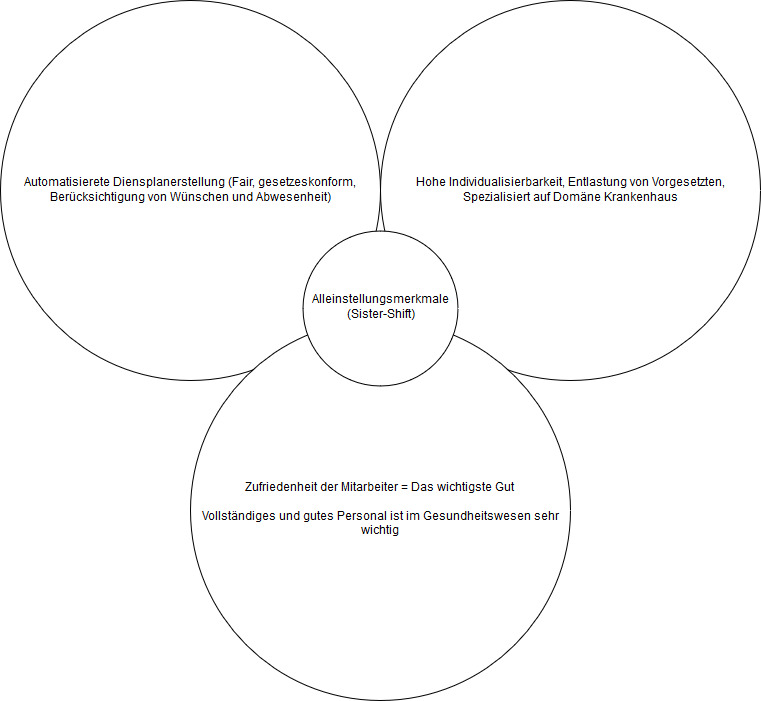
\includegraphics[scale=0.45]{Bilder/USP.jpg}{\centering}
\caption{Sister Shift Alleinstellungsmerkmale}
\end{figure}
\section{Vorgehensmodell}
Die Anwendung Sister-Shift hat zum größten Teil einen gesellschaftlichen Nutzen. Die strategischen Ziele sind ganz klar die Entlastung der Stationsleitung, die Vereinfachung der Einsatz-/Abwesenheitsplanung und am wichtigsten, die faire Behandlung beim Thema Arbeitszeit/Schichtplanung aller Gesundheits- und Krankenpfleger in einem Krankenhaus. Zusätzlich sollen die Mitarbeiter die Möglichkeit haben, Ihre Einsatzpläne mit Einschränkungen zu Individualisieren. Dafür müssen diese gut mit der Anwendung umgehen können. Über lange Zeit gesehen, verbessert dies die Zufriedenheit und steigert somit auch die Arbeitsmoral der Arbeitnehmer. Letztendlich kommt diese Verbesserung der Zufriedenheit und Moral auch den Patienten zu Gute. Da Arbeitnehmer die wichtigste Ressource in einer Organisation sind, kommen die Verbesserungen auch dem Krankenhaus selbst zu Gute. Aus den genannten Gründen hat das Wohlbefinden der Arbeitnehmer in einem Unternehmen, beziehungsweise in einer Organisation, eine sehr hohe Priorität. 
Da bei der Entwicklung der Anwendung Sister-Shift ganz klar die Mitarbeiter und deren Dienstplanung im Fokus stehen, wird die Anwendung entlang des Menschzentrierten Entwicklungsprozess entwickelt. Als Vorgehensmodell wird das Wasserfall- Modell verfolgt. Die Anforderungen an das System, die daraus resultieren, unterstützen tatsächlich den Nutzer. 
\begin{figure}[h]
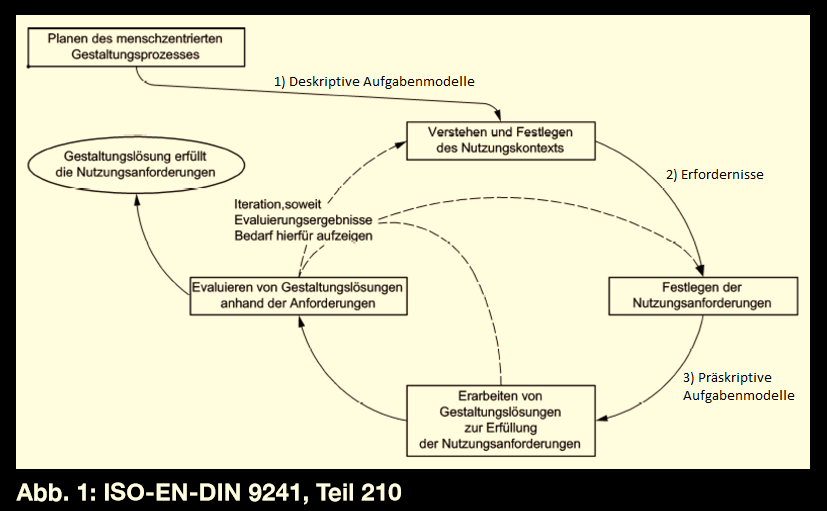
\includegraphics[scale=0.55]{Bilder/Vorgehensmodell.png}{\centering}
\caption{Der menschzentrierte Entwicklungsprozess}{\centering}
\end{figure}

Die Grundsätze der menschzentrierten Gestaltung sind zum einen ein umfassendes Verständnis der Benutzer, deren Arbeitsaufgaben und Umgebung, der Einbezug der Benutzer, die Berücksichtigung der User Experience, Einfluss fachübergreifender Kenntnisse und das ständige Iterieren der Entwicklungsschritte. Durch diese Grundsätze soll ein interaktives System gebrauchstauglicher gemacht werden.
Alles zusammen führt dies zu einer Steigerung der Produktivität und Zufriedenheit. Es führt außerdem zu einem gesteigerten Wohlbefinden des Nutzers und der Vermeidung von Stress. Eine erhöhte Zugänglichkeit und vermindertes Risiko physischer und psychischer Belastung sind zusätzliche Wirkungen der menschzentrieren Entwicklung. Zuletzt wird bei dieser Vorgehensweise auch die Lernförderlichkeit und User Experience verbessert.
Die genannten Aspekte führen zusammengefasst zu einer Verbessrung der Arbeit des jeweiligen Arbeitnehmers. 
Das Rahmenmodell der Menschzentrierten passt auf Grund der genannten Wirkungen exzellent zu dem Entwicklungsprozess der Anwendung Sister-Shift.
Als konkretes Vorgehensmodell dient das Wasserfall-Modell. Die strikte Reihenfolge ist dabei das ausschlaggebende Argument. Zuerst muss die Domäne des Krankenhauses bzw. die Organisation der Einsatzzeiten in diesem verstanden werden. Ist dies geschehen, werden die Anforderungen an das System definiert. Sobald die Anforderungen aufgestellt sind, folgen Überlegungen zur Gestaltung der Software. Dabei wird sowohl die Software-Architektur, als wie auch das spätere Userinterface berücksichtigt. Sind alle erforderlichen Gestaltungsentscheidungen getroffen, ordentlich modelliert und begründet, so wird die Software implementiert. Nach der Implementierung erfolgt eine umfassende Evaluation der Arbeit. Sind alle Erfordernisse und Kriterien erfüllt, so geht das Projekt in die letzte Phase der Instandhaltung über.
\begin{figure}[h]
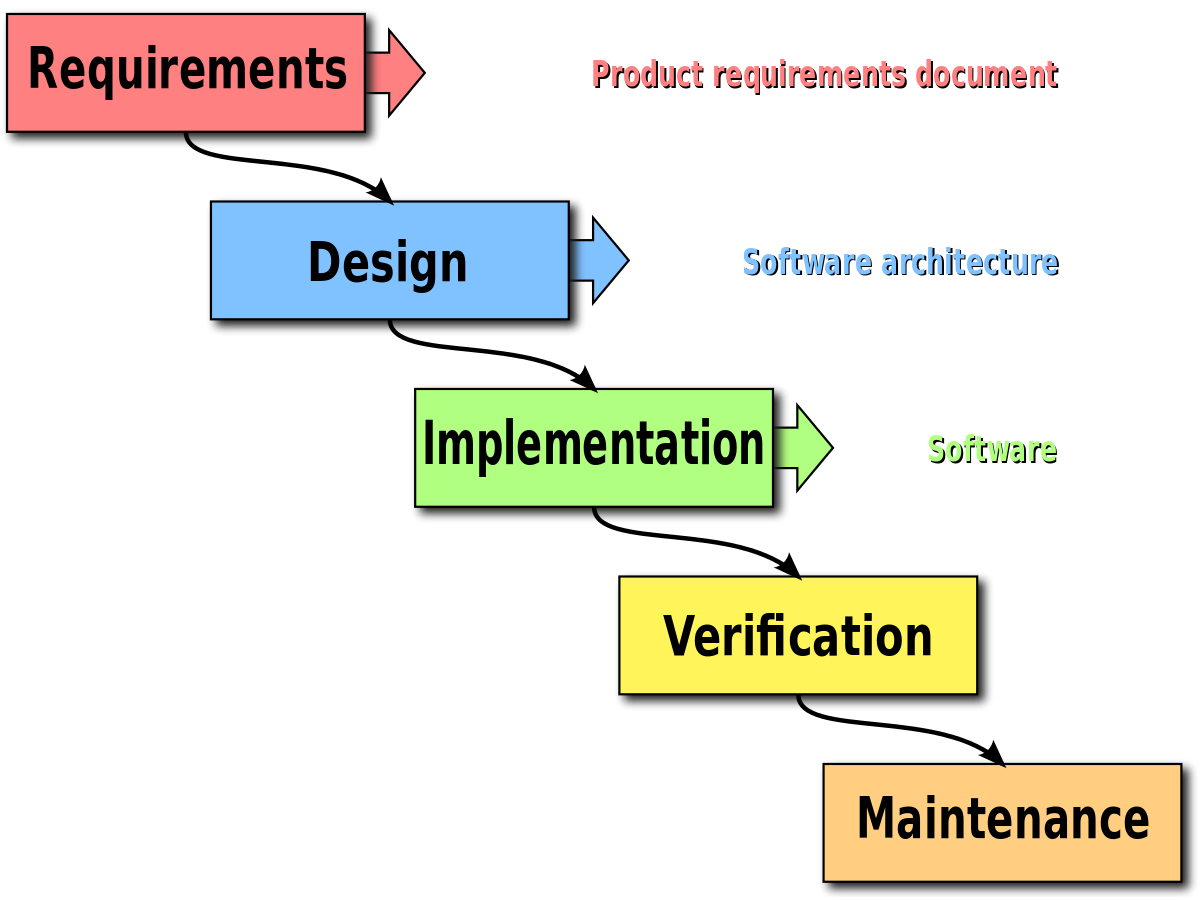
\includegraphics[scale=0.39]{Bilder/1200px-Waterfall_model.jpg}{\centering}
\caption{Waterfall-Model}
\end{figure}
\section{Kommunikationsmodelle}
\subsection{Deskriptives Modell}
\begin{figure}[H]
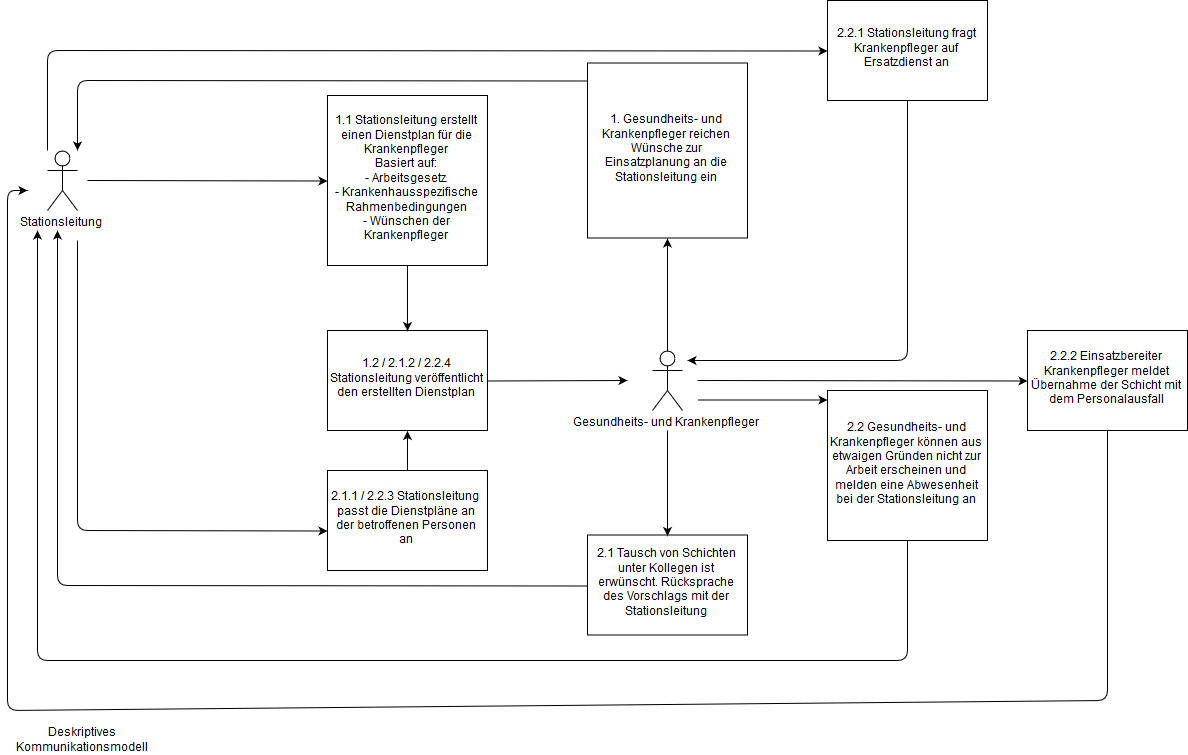
\includegraphics[scale=0.3]{Bilder/KommunikationsmodellierungDeskriptiv.jpg}{\centering}
\caption{Deskriptives Modell}
\end{figure}
Zu sehen ist das deskriptive Kommunikationsmodell bezüglich der Dienstplanerstellung und Organisation von Schichttausch und Ersatzplanung. Man kann dem Modell entnehmen, dass die Stationsleitung ein wichtiger Knotenpunkt bei der Erledigung der genannten Aufgaben ist. Die Stationsleitung muss bei jeder Aufgabe einzeln mit den Gesundheits- und Krankenpflegern kommunizieren, und ist drauf angewiesen, dass diese auch gut erreichbar sind beziehungsweise gut an der Kommunikation mitwirken, damit alle erforderlichen Informationen auch schnell und korrekt zur Verfügung stehen. Bei Abwesenheitsmeldungen oder zu vielen Anfragen auf Schichtänderungen, kommt die Stationsleitung schnell in eine Stresssituation.  Bei einem Personalausfall muss manuell, über Rücksprachen mit den anderen Krankenpflegern, ein Ersatz ermittelt, eingesetzt und der betroffene Dienstplan abgeändert werden. Eine Unterbesetzung in einem Krankenhaus ist nicht geduldet und darf nicht auftreten. Anfragen auf Schichtänderungen belasten die Stationsleitung zusätzlich, und zwingen diese, wiederum mit den betroffenen Krankenpflegern zu kommunizieren und die Dienstpläne manuell zu ändern. 
Das geplante System, soll die Stationsleitung um die Aufgabe der Dienstplanerstellung, und die restliche genannte Organisation erleichtern. Ein großer Teil der umständlichen Kommunikation soll entfallen.
\subsection{Präskriptives Modell}
\begin{figure}[H]
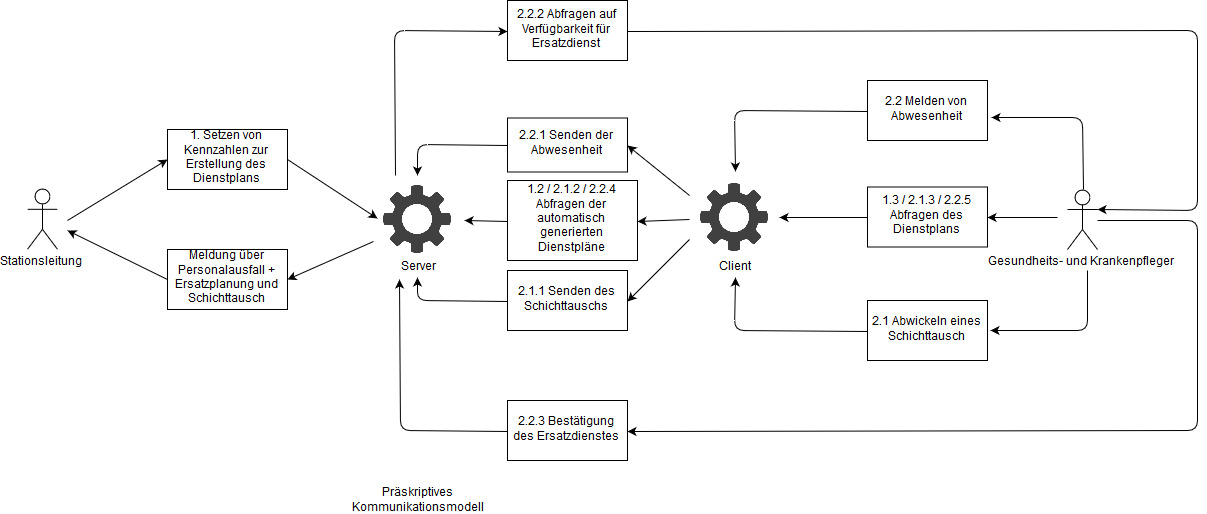
\includegraphics[scale=0.3]{Bilder/PraeskriptivesKommunikationsmodell.jpg}{\centering}
\caption{Präskriptives Modell}
\end{figure}
Abbildung 2 beschreibt das präskriptive Kommunikationsmodell, nach Einsatz des geplanten Systems. Die Aufgabe der Dienstplanerstellung wurde an das System übertragen. Zusätzlich entfällt die Umständliche Kommunikation mit jedem einzelnen Krankenpfleger, da diese über das System selbstständig Abwesenheitsmeldungen und Tauschanfragen bezüglich einer Schicht einreichen können. Das System verarbeitet die Informationen und plant den Ersatz oder tauscht die Schicht und ändert automatisch die Dienstpläne. Es informiert die Stationsleitung über alle Personalausfälle und vollzogenen Schichttausche.
\section{Aufgabenmodellierung}
\subsection{Deskriptive Aufgabenmodellierung}
Methode: HTA (Hierarchical Task Analysis)
\begin{figure}[H]
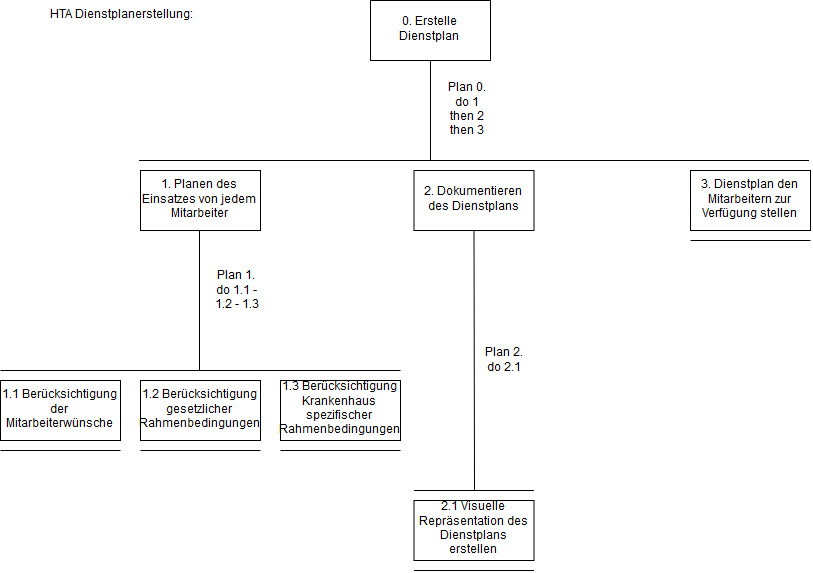
\includegraphics[scale=0.4]{Bilder/Dienstplanerstellung.jpg}{\centering}
\caption{HTA Dienstplanerstellung}
\vspace{3cm}
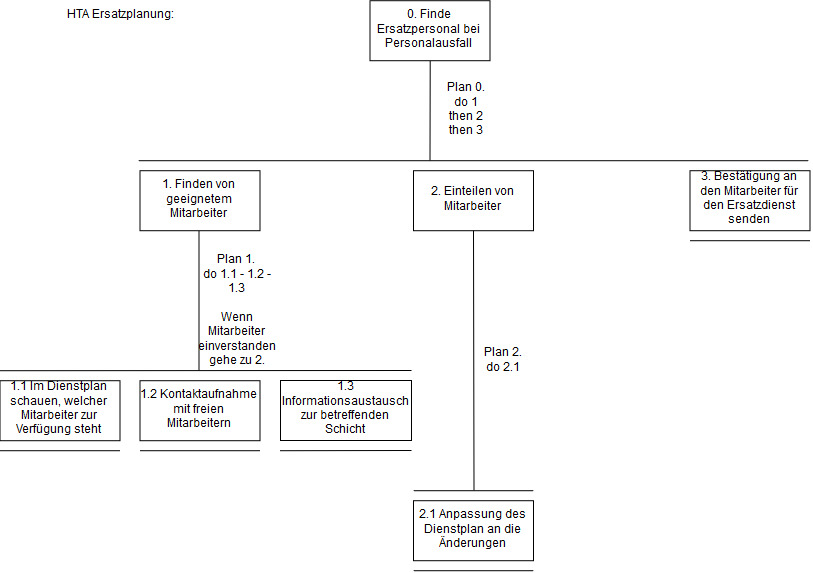
\includegraphics[scale=0.4]{Bilder/Ersatzplanung.jpg}{\centering}
\caption{HTA Ersatzplanung}
\end{figure}
\begin{figure}[h]

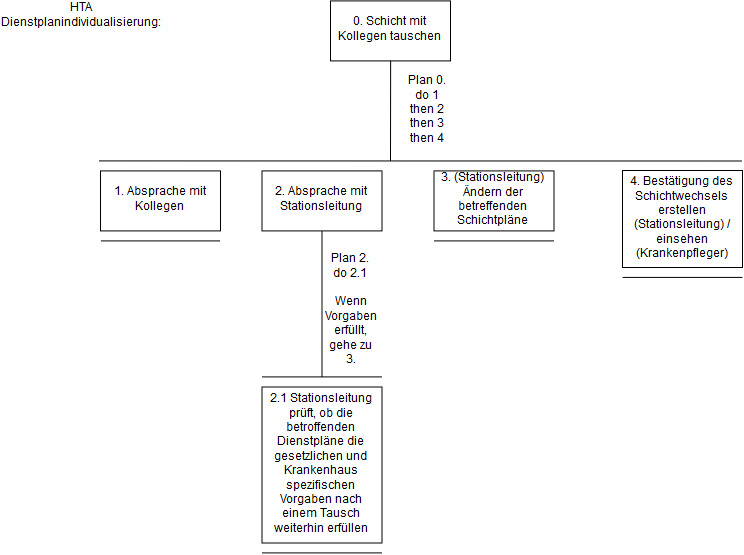
\includegraphics[scale=0.4]{Bilder/Individualisierung.jpg}{\centering}
\caption{HTA Dienstplanindividualisierung}

\end{figure}
\subsection{SWOT Analyse}
\subsubsection{Strengths}
Die Dienstplanerstellung erfolgt manuell, wodurch eine permanente Kontrolle auf Konformität des Dienstplans durch eine Person gewährleistet ist.  Wünsche können individuell und mit besonderer Priorität in den Dienstplan eingepflegt werden. Es herrscht bei der Dienstplanerstellung stets Kommunikation zwischen Krankenpflegern und Stationsleitung.
\subsubsection{Weaknesses}
Der Aspekt des Manuellen Dienstplanschreibens ist auch eine Schwäche. Für die Erstellung des Dienstplans wird eine Menge Zeit benötigt. Diese Zeit könnte man besser in das Wohlergehen der Patienten oder anderen in dem Zusammenhang stehenden Aufgaben investieren. Zudem ist es sehr schwer einen fairen Dienstplan für alle Mitarbeiter zu erstellen.
Die fehlende Organisation bei der Ersatzplanung ist eine große Schwäche. Die Stationsleitung muss manuell die zur Verfügung stehenden Mitarbeiter ermitteln, und anschließend kontaktieren. Wenn ein Ersatz gefunden ist, muss ebenfalls manuell, der Dienstplan der betroffenen Person angepasst werden. Das ganze Vorgehen kostet sehr viel Zeit und Mühen. Meistens müssen die Krankenpfleger sogar selbst bei der Organisation von Ersatz mithelfen, was dieses zusätzlich belastet. Falls kein Ersatz gefunden wird, kann es zu einer Unterbesetzung kommen. Dieses Risiko kann sich auf die Patienten auswirken.
Eine weitere Schwäche ist die fehlende Individualisierbarkeit der Dienstpläne, welche von den Krankenpflegern selbst geschieht. Schichtwechsel sind nur über die Stationsleitung möglich, welche dieses wieder viel Arbeit und Mühen kosten.
\subsubsection{Opportunities}
Mit der Anwendung des einzusetzenden Systems ergeben sich eine Menge Vorteile. Die automatische Dienstplanerstellung entlastet die Stationsleitung ungemein und sorgt für eine große Zeitersparnis. Die Stationsleitung kann sich dementsprechend anderen Aufgaben widmen. Bei dem automatisierten Erstellen der Dienstpläne wird zusätzlich ein möglichst fairer Plan für alle erstellt. Diese Tatsache steigert die Arbeitsmoral der Gesundheits- und Krankenpfleger, wodurch ebenfalls die Patienten profitieren. 
Das Organisieren von Ersatz bei Personalausfällen erfolgt ebenfalls automatisch. Die in Frage kommenden Mitarbeiter werden zudem nur minimal in die Organisation eingebunden. Dies erspart sowohl der Stationsleitung, als auch den Gesundheits- und Krankenpflegern eine Menge Stress, Arbeit und Zeit. 
Ein weiterer entlastender Aspekt bietet die Möglichkeit des Schichtentauschs. Die Krankenpfleger können Ihre Schichten mit Hilfe der Anwendung eigenständig, also ohne Einbindung der Stationsleitung tauschen. Die Möglichkeit für einen Schichttausch steigert sowohl die Moral der Krankenpfleger, entlastet aber zugleich auch die Stationsleitung, da diese nicht mehr manuell die Dienstpläne anpassen muss. 
\subsubsection{Threats}
Durch das automatische Erstellen der Dienstpläne ergeben sich allerdings auch ein paar Gefahren. So kann es zum Beispiel sein, dass Wünsche nicht immer beachtet werden. Arbeitet Krankenpfleger X gerne mit Krankenpfleger Y zusammen, so kann es sein, dass diese auf Grund der fairen Dienstplanerstellung nicht zusammen eingeteilt werden.
Eine weitere Gefahr bietet die Organisation des Ersatzes im Falle eines Personalausfalls. Wenn sich kein Mitarbeiter bereit erklärt einzuspringen, beziehungsweise keiner der Mitarbeiter auf Grund der Gesetzeslage fähig ist die betroffene Schicht zu übernehmen, so müssen Alternativen gefunden werden.
Auf Grund der Möglichkeit, dass Mitarbeiter Ihre Schichten untereinander unabhängig tauschen können, kann es passieren, dass die Stationsleitung den Überblick über das eingeteilte Personal verliert. Dies sollte im Regelfall allerdings nicht passieren, da die Anwendung viel mit der Stationsleitung kommuniziert und diese bei Änderungen benachrichtigt.
\subsection{Präskriptive Aufgabenmodellierung}
Methode: HTA (Hierarchical Task Analysis)
\begin{figure}[H]
\includegraphics[scale=0.45]{Bilder/DPerstellung.jpg}{\centering}
\caption{HTA Dienstplanerstellung (Präskriptive)}
\vspace{3cm}
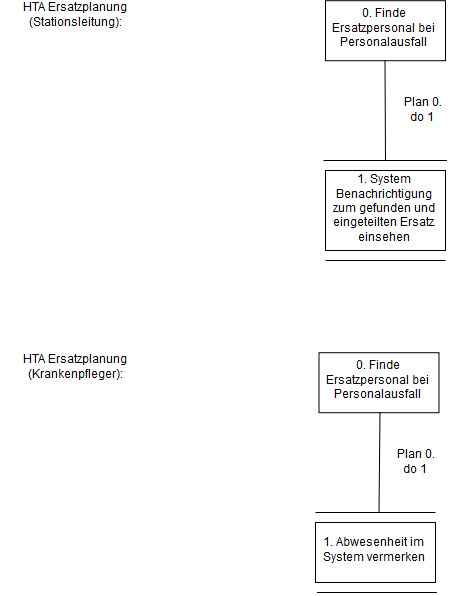
\includegraphics[scale=0.55]{Bilder/ersatzplanungP.jpg}{\centering}
\caption{HTA Ersatzplanung (Präskriptive)}
\vspace{3cm}
\end{figure}
\begin{figure}[h]
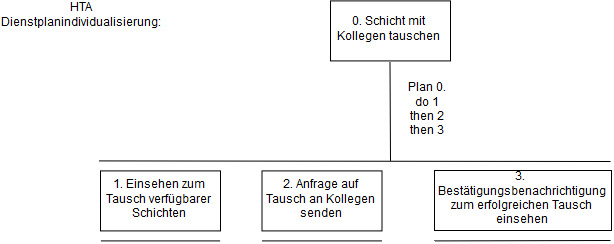
\includegraphics[scale=0.5]{Bilder/IndiPraes.jpg}{\centering}
\caption{HTA Dienstplanindividualisierung}
\end{figure}
\section{Systemarchitektur}
Im Folgenden werden die Vor- und Nachteile eines zentralen und eines dezentralen Architektur Stils anhand von Beispielen diskutiert.
\subsection{Systembegründung}
\subsubsection{Client-Server}
Das Client – Server System basiert auf einem zentralen Stil. Bei dieser Orchestrierung übernimmt der Server die Rolle des Dirigenten. Der Client hingegen steht dem Server als Musiker entgegen. Im genaueren heißt das, dass der Server eine oder mehrere Schnittstellen besitzt über diese Daten vom Client/-s empfangen oder gesendet werden. Der Client kann Informationen anfragen und diese darauf weiterverarbeiten. Hierbei übernimmt der Server die Datenhaltung, wodurch die Redundanz von Ressourcen vermieden werden kann. Der Ausfall eines Clients im System ist leicht zu verkraften, fällt hingegen die Serverkomponente aus, sind alle Clients betroffen. Diese könnten nur noch beschränkt oder gar nicht ausgeführt werden. Deshalb ist es empfehlenswert einen redundant arbeitenden Server zu installieren, um die Ausfallmöglichkeit des Systems zu dezimieren.
\subsubsection{Peer to Peer}
Die Peer to Peer Architektur ist anders als die Client – Server Architektur ein dezentrales System. Hierbei können die Systemkomponenten Dienste und Ressourcen bereitstellen, aber genauso auch auf diese Zugreifen. Dies ist besonders Organisationsbedürftig, um Redundanz zu vermeiden und ein möglichst effizientes System zu schaffen, müssen die Dienste und Ressourcen genau strukturiert und an die einzelnen Systemkomponenten sinnvoll verteilt werden. Es ist nicht aussenvor zu lassen, dass die Ausfallsicherheit bei diesem Stil sehr hoch ist.
\subsubsection{Fazit}
Nach Abwägung der Architekturen, kann beim Adaptieren mit dem vorliegenden Projekt, der Schluss gefasst werden, dass eine Peer to Peer Architektur ungeeignet ist. In unserer Domäne erfüllt die Stationsleitung die zentrale Rolle der Dienstplanerstellung. Ein gemeinsames Erstellen des Dienstplans, würde zu einem Chaos führen. Das Client-Server Modell spiegelt die Rollenverteilung zwischen Stationsleitung und Krankenpflegern wieder. Zudem verfügt dieser Stil über eine klare Verteilung der Anwendungslogik, welche die Verantwortung und Last der Funktionalität verteilt. In der Projektdomäne ist es notwendig, dass ein Client an einer zentralen Stelle, alle für ihn wichtigen Informationen erhält.
\subsection{Architekturstil REST}
Im Folgenden wird erläutert, warum der Architekturstil REST für das Projekt Sister Shift gewählt wurde.
\subsubsection{Lose Kopplung}
Dadurch das die Systemkomponenten über Schnittstellen kommunizieren, können die Teilkomponenten leichter aktualisiert, modifiziert, außer Betrieb genommen oder ersetzt werden. Anders als bei monolithischen Systemen, können Teilkomponenten ausfallen, ohne dass, das gesamte System zusammenbricht. Sister Shift profitiert hierbei besonders, da zuvor genannten domänenspezifische und gesetzliche Vorgaben zur Einsatzplanung leicht aktualisiert werden können.
\subsubsection{Interoperabilität}
Es ist möglich mit technisch stark unterschiedlichen Systemen zu kommunizieren. Über gemeinsame Standards wie, HTTP, URIs,
JSON, XML oder HTML können unterschiedliche Systeme Informationen austauschen. Hierbei ist auch das HTTP bzw. HTTPS Protokoll und die URIs als Identifikationsmechanismus relevant. Funktionen wie das eintragen der Wünsche, oder das erstellen einer Krankmeldung, sowie auch andere Funktionen spiegeln die Semantik der HTTP Methoden wieder.
\subsubsection{Wiederverwendbarkeit}
Da es bei REST nur eine Schnittstelle gibt, kann jedes System, dass diese Schnittstelle kennt, mit dem REST-Service kommunizieren. Die Problemdomäne der Arbeitsplanung in der Schichtarbeit tritt nicht nur im Gesundheitswesen auf, deswegen kann in zukünftigen Projekten Sister Shift als Basis für solche Projekte dienen. 
\subsubsection{Performance und Skalierbarkeit}
Da bei Rest über HTTP kommuniziert wird und auf einen sitzungsbezogenen Status verzichtet wird, entsteht ein positiver Effekt bezüglich der Skalierbarkeit. Egal ob Sister Shift für nur ein Krankenhaus oder in allen Krankenhäusern deutschlandweit zur Verfügung steht, wird immer performant auf eine serverseitige Anfrage geantwortet
\begin{figure}[H]
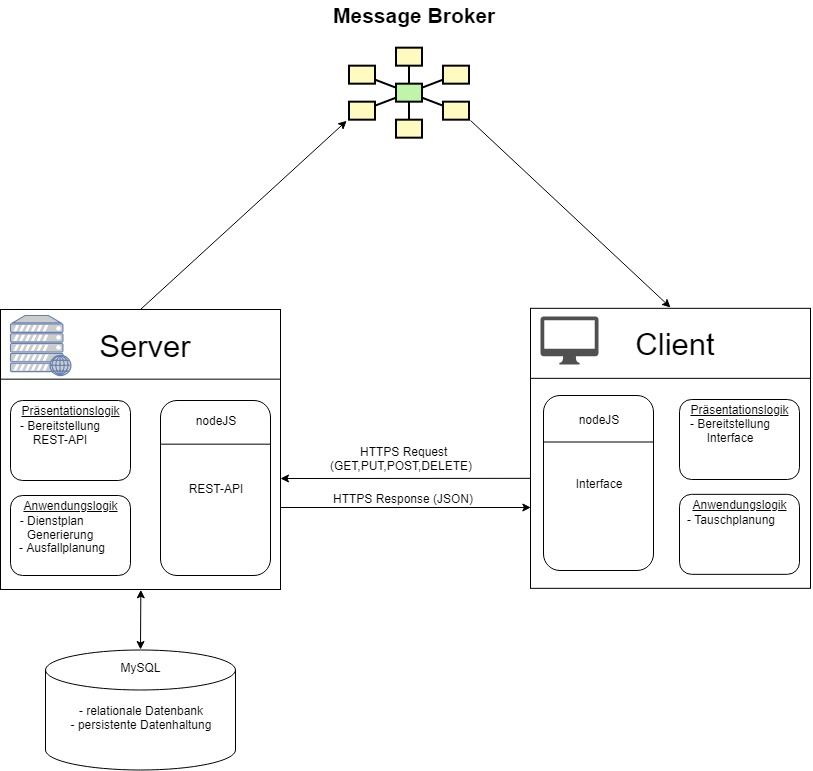
\includegraphics[scale=0.45]{Bilder/Architekturdiagramm.jpg}{\centering}
\caption{Architekturdiagramm}
\end{figure}
\subsection{Systemkomponenten}
\subsubsection{Server}
Der Server stellt die zentrale Schnittstelle der Anwendung dar. Er stellt eine REST-API bereit mit der die Clients kommunizieren. Die REST-API wird mithilfe von nodeJS umgesetzt, Ressourcen sind hiermit leicht zu implementieren. Mithilfe von Client Informationen sollen hier automatisiert Dienstpläne erstellt werden und auf Ausfälle entsprechend reagiert werden.
\subsubsection{Client}
Der Client stellt ein Interface dar, dass mit dem Server kommuniziert. Implementiert wird der Client in nodeJS oder Java, je nachdem ob es sich um eine Webportal oder eine mobile Applikation handelt.
Der Client soll mit Hilfe von Serverinformationen geeignete Schichten zum Tauschen identifizieren und diese an den Server übermitteln.
\subsubsection{Message Broker}
Der Message Broker übernimmt die Aufgabe des Benachrichtigens der Clients. Der Server wartet auf einen spezifischen Zustand. Tritt dieser ein, setzt er eine Nachricht inklusive Schlüssel an den Message Broker ab. Dieser stellt mit Hilfe des Schlüssels fest welche Clients eine Benachrichtigung erhalten sollen und übermittelt die Nachricht.
\subsubsection{Datenhaltung}
Die Daten werden auf dem Server in einer relationalen Datenbank, die auf MySQL basiert persistent gespeichert.
\subsubsection{Kommunikation}
Die Kommunikation verläuft asynchron über das verschlüsselte HTTPS Protokoll. Server und Client nutzen zur Datenübertragung das JSON Format. Die Kommunikation zwischen Client und Message Broker verläuft ebenfalls asynchron.
\section{Risikoanalyse}
Aus den identifizierten Alleinstellungsmerkmalen und der Zielsetzung, werden im folgenden Abschnitt Risiken identifiziert. Dabei werden, sofern möglich, entsprechende Gegenmaßnahmen geplant.
\subsection{Allgemeine Risiken}
\subsubsection{Bereitschaft der Gesundheits- und Krankenpfleger}
Bereitschaft der Gesundheits- und Krankenpfleger ein neues System zur Dienstplanung zu verwenden. Damit ist inbegriffen, das Einsehen der Dienstpläne, das Tauschen von Schichten und das Melden von Abwesenheit.
\subsubsection{Unzufriedenheit}
Unzufriedenheit mit den erstellten Dienstplänen, welche automatisiert durch das System erstellt wurden.
\subsection{Projektspezifische Risiken}
\subsubsection{Rückmeldung auf Abwesenheitsmeldung}
Es kann zu der Situation kommen, dass die Gesundheits- und Krankenpfleger, eine Übernahmeanfrage einer Schicht zu spät oder gar nicht beantworten. Da es in einem Krankenhaus keinen Personalmangel geben darf, muss diesem Fall vorgebeugt werden. Tritt der genannte Fall ein, so wird das System automatisch eine Zeitarbeitsfirma kontaktieren, und dieser alle Informationen übermitteln.
\subsubsection{Simultane Rückmeldung auf Ersatzanfrage}
Tritt der Fall ein, dass sich mehr als ein Krankpfleger gleichzeitig zur Übernahme einer Schicht bereiterklären, kann es zu Zuweisungskonflikten kommen. Dieser Fall wird mit Hilfe von exklusivem Zugriff, welcher durch einen Semaphor gewährleistet wird, abgedeckt.
\subsubsection{Schichtentausch}
Bei einem Schichttausch kann es passieren, dass der Dienstplan nach dem Tausch gegen gesetzliche oder domänenspezifische Rahmenbedingungen verstößt. Das System prüft anhand des vorhandenen Dienstplanes, ob der gewünschte Tausch die Bedingungen erfüllt.
\subsubsection{Benachrichtigen bei Abwesenheitsmeldung}
Bei einer Abwesenheitsmeldung, sollen nicht alle Krankenpfleger des Krankenhauses informiert werden, sondern nur die, welche auch als Ersatz in Frage kommen. Das System selektiert anhand von der Station und des bestehenden Dienstplanes die passenden Personen.
\subsubsection{Wünsche zur Einsatzplanung}
Bei dem automatischen Erstellen eines Dienstplanes, werden nicht immer die Wünsche von allen Krankenpflegern berücksichtigt. Das System ermittelt über ein Rating, welche Wünsche bevorzugt mit in den Einsatzplanung einfließen.
\section{Proof of Concept}
Im Folgenden wird beschrieben, wie das System mit den identifizierten Risiken umgeht.
\subsection{Rückmeldung auf Abwesenheitsmeldung}
Ein Krankenpfleger soll sich auf eine Ersatzanfrage zurückmelden.
\subsubsection{Exit:}
Ein Krankenpfleger hat sich erfolgreich als Ersatz gemeldet und wurde eingeteilt.
\subsubsection{Fail:}
Die verfügbaren Krankenpfleger haben sich nicht oder zu spät zurückgemeldet.
\subsubsection{Fallback:}
Es ist wichtig, dass alle Schichten durchgängig voll besetzt sind. Im erfolgslosen Fall wird eine Zeitarbeitsfirma kontaktiert.
\subsection{Simultane Rückmeldung auf Ersatzanfrage}
Ein Krankenpfleger soll sich auf eine Ersatzanfrage zurückmelden.
\subsubsection{Exit:}
Nur ein Krankenpfleger hat sich erfolgreich als Ersatz gemeldet und wurde eingeteilt.
\subsubsection{Fail:}
Mehr als ein Krankenpfleger melden sich simultan als Ersatz an.
\subsubsection{Fallback:}
Es ist wichtig, dass der Zugriff auf die Rückmeldung exklusiv ist und sich somit nur ein Krankenpfleger gleichzeitig als Ersatz melden kann. Dies wird durch ein Semaphor gewährleistet.
\subsection{Schichtentausch}
Ein Krankenpfleger möchte seine Schicht mit einem anderen tauschen.
\subsubsection{Exit:}
Der Tausch verstößt gegen keine gesetzlichen oder domänenspezifische Rahmenbedingungen.
\subsubsection{Fail:}
Der Tausch verstößt gegen die genannten Rahmenbedingungen, und kann nicht erfolgen.
\subsubsection{Fallback:}
Es ist wichtig, dass ein Tausch die genannten Bedingungen berücksichtigt. Das System prüft dies, und lässt einen Tausch nur bei Erfolg zu.
\subsection{Benachrichtigen bei Abwesenheitsmeldung}
Ein Krankenpfleger meldet eine Abwesenheit.
\subsubsection{Exit:}
Alle Krankenpfleger die als Ersatz in Frage kommen werden benachrichtigt. 
\subsubsection{Fail:}
Mehr als nur die in Frage kommenden Krankenpfleger werden informiert.
\subsubsection{Fallback:}
Es ist wichtig, dass nur die Krankenpfleger, welche die Schicht mit dem Personalausfall übernehmen können, benachrichtig werden. Dies wird über eine Selektion der Krankenpfleger, bezüglich Station und gegebenem Dienstplan gewährleistet.
\subsection{Wünsche zur Einsatzplanung}
Ein Krankenpfleger teilt einen Wunsch zur Einsatzplanung mit.
\subsubsection{Exit:}
Der Dienstplan beinhaltet den Wunsch. 
\subsubsection{Fail:}
Der Wunsch wurde in der Dienstplanerstellung nicht berücksichtigt.
\subsubsection{Fallback:}
Es ist wichtig, dass Krankenpfleger Wünsche zur Einsatzplanung äußern können. Die Berücksichtigung dieser ist nicht immer gewährleistet. Das System verteilt den Grad der Berücksichtigung durch ein Rating fair auf alle Krankenpfleger.
\end{document}